
%(BEGIN_QUESTION)
% Copyright 2006, Tony R. Kuphaldt, released under the Creative Commons Attribution License (v 1.0)
% This means you may do almost anything with this work of mine, so long as you give me proper credit

How much pressure is being applied to this U-tube water manometer, in units of ``inches of water column'' and ``pounds per square inch''?

$$\includegraphics[width=15.5cm]{i00161x01.eps}$$

What would happen to the liquid levels if the water were replaced by an oil with a lesser {\it density}?  Given the same applied pressure, would the distance between the two liquid columns be greater, less, or the same as shown in the above illustration?

\underbar{file i00161}
%(END_QUESTION)





%(BEGIN_ANSWER)

Applied pressure = 9 "W.C., which is equal to 0.32514 PSI.

\vskip 10pt

For the same applied pressure, the distance between the two liquid columns will be {\it greater} than with water.  In other words, for a pressure of 9" W.C., there will be {\it more} than 9 inches of vertical distance separating the two liquid columns.

Essentially, manometers work on the principle of balanced pressures: the applied gas pressure forces the liquid columns to shift height.  When they do so, they generate a hydrostatic pressure proportional to their differential height.  When this hydrostatic pressure equals the applied pressure, the liquid columns stop moving and a condition of equilibrium is reached.

If a lighter fluid such as oil is used instead of water, a greater height will have to be developed to generate the same amount of hydrostatic pressure to oppose the applied gas pressure and reach equilibrium.  Conversely, if a heavier (denser) liquid such as mercury were to be used, a much smaller vertical height would develop between the two columns for the same pressure.

%(END_ANSWER)





%(BEGIN_NOTES)


%INDEX% Measurement, pressure: manometer

%(END_NOTES)


